\chapter{数据同步与平滑机制的设计与实现}
系统测试是为了在用户开始使用软件前,尽可能地发现软件中潜在的错误
和不合理之处,确保最后将高质量的软件交付给用户。为了验证系统的功能和
性能是否与需求分析时的规格说明一致,本章节在开发环境和真实FFS环境中分别做综合性的功能测试和性能测试。

\section{开发PC环境测试}
由于国内的FFS全部位于航空公司的训练基地内,不具备移动的可能性,平日开发过程中的测试均使用虚拟仿真机读取模拟数据,并在开发PC上完成视景渲染。
受限于硬件性能,在开发环境下的测试以功能测试为主,确保功能正常运作即可,对于画面帧率和分辨率之类不做严格要求。
\subsection{测试环境}
在开发环境下,虚拟仿真机由笔记本电脑担任,模拟数据也位于该电脑上,在Windows系统上运行程序,便可以通过Tbuspp与视景建立连接,不断地读取并发送数据。
对于运行视景的机器有较高的硬件要求,GPU部分要使用较高型号才能让开发人员流畅的观察场景。同时由于搭载了大型机场场景数据库,对于硬盘容量也有较高要求。在测试环境的具体物理配置信息如表\ref{devhard}所示。
\begin{table}[h!]
    \begin{center}
        \caption{开发环境物理配置}
        \renewcommand\arraystretch{1.5}
        \label{devhard}
        \begin{tabularx}{\textwidth}{ 
             >{\centering\arraybackslash\hsize=.4\hsize\linewidth=\hsize}X 
             >{\centering\arraybackslash\hsize=.4\hsize\linewidth=\hsize}X 
             >{\centering\arraybackslash\hsize=\hsize\linewidth=\hsize}X 
             }
             \hline
            \textbf{设备} & \textbf{配置项} & \textbf{详情}\\
             \hline
             & CPU & AMD Ryzen 7 4700G 8-Core Processor\\
           
             & GPU & NVIDIA GeForce RTX 3060\\
             
             视景运行机 & 内存 & 32GB\\
            
             & 硬盘 & 8TB\\
             
             & 系统 & Windows 10 专业版 22H2\\
             \hline
             & CPU & AMD Ryzen 7 5800H with Radeon Graphics\\
           
             & GPU & AMD Radeon(TM) Graphics\\
             
             虚拟仿真机 & 内存 & 16GB\\
            
             & 硬盘 & 512GB\\
             
             & 系统 & Windows 10 专业版 22H2\\
             \hline
            \end{tabularx}
    \end{center}
\end{table}
\par
为了顺利运行系统,服务器上需要配置系统运行的软件环境,详细信息如表\ref{devsoft}所示。
开发PC测试环境下的软件要求与真实FFS下的测试相同,后不再赘述。两方都需要C++与Python的运行环境,且双方通过Tbuspp沟通。
在虚拟仿真机中,需要与仿真机进行直接的链路层信息交流,需使用WinPcap软件。测试环境部署配置完成后应当能保证系统不会因为环境问题出错。

\begin{table}[h!]
    \begin{center}
        \caption{开发环境软件配置情况}
        \label{devsoft}
        \renewcommand\arraystretch{1.5}
        \begin{tabularx}{0.8\textwidth}{ 
             >{\centering\arraybackslash\hsize=.5\hsize\linewidth=\hsize}X 
             >{\centering\arraybackslash\hsize=\hsize\linewidth=\hsize}X 
             }
             \hline
            \textbf{配置项 } & \textbf{详情}\\
             \hline
             C++运行环境 & VS\_C++\_MSVC\\
           
             Python运行环境 & Python\thinspace 3.10\\
             
             底层网络访问 & WinpCap\thinspace v4.1.3\\
            
             服务网格 & Tbuspp \thinspace 0.6.0\\
             \hline
            \end{tabularx}
    \end{center}
\end{table}
\subsection{功能测试}
对于本系统的功能测试而言,视景中的飞机能够按照模拟数据中的路径飞行,即可说明从数据读取到协议转换再到最后的信息发送功能都是通过测试的。
\par 
图\ref{synctest}是对频率限制工具FrameFrequencyRestriction测试的效果,测试过程中将其频率设置为30Hz,运行csv文件读取部分程序,
可以看到从读取第18行数据到读取第48行数据中正好间隔1秒钟。多种频率均能通过测试。
\clearpage
\begin{figure}[h!]
    \begin{center}
        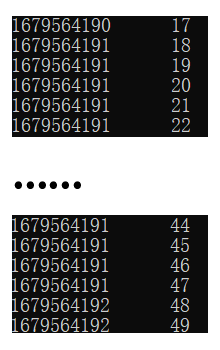
\includegraphics[width=0.4\textwidth]{pictures/frame.png}
        \caption{30HZ频率限制效果}
        \label{synctest}
    \end{center}
\end{figure}
\par
我们在测试中使用到的模拟数据是飞行员在训练基地FFS上操作绕深圳宝安机场飞行一周后得到的数据。
该数据的采样频率为60Hz,共6万余组数据,每组数据中包含仿真机输出的原始经纬高和欧拉角信息。
首先测试经过虚拟仿真机发送给游戏引擎的数据是否正确,采用的方法是在GIS软件中绘制这组输出数据,查看绘制路径与飞行员的飞行路径是否相同。
图\ref{GIStrace}中的轨迹是由上述原始数据经过虚拟仿真机处理最终输出的6万个点构成,可以看到轨迹起始位置精确的位于宝安机场的跑道上,
起飞后环绕深圳市区飞行,最终截止于羊台山森林公园。与飞行员核对后确认本路径准确无误,说明由仿真机到游戏引擎中间一系列数据操作均可以通过测试。

\par
在确认虚拟仿真机输出无误后,便可使用此数据进一步测试游戏引擎中飞行控制逻辑。图\ref{firsttest}是飞机第一视角下的飞行画面,可以看到根据模拟数据,飞机准确出现在宝安机场跑道上,
且后续飞行中的爬升转向时的视角偏转完全符合实际情况,最终飞机按照轨迹终止于场景中的森林公园上空。此测试过程同样表明第一视角摄像机可以正确跟随飞机位置并做出相同的姿态。
\clearpage
\begin{figure}[h!]
    \begin{center}
        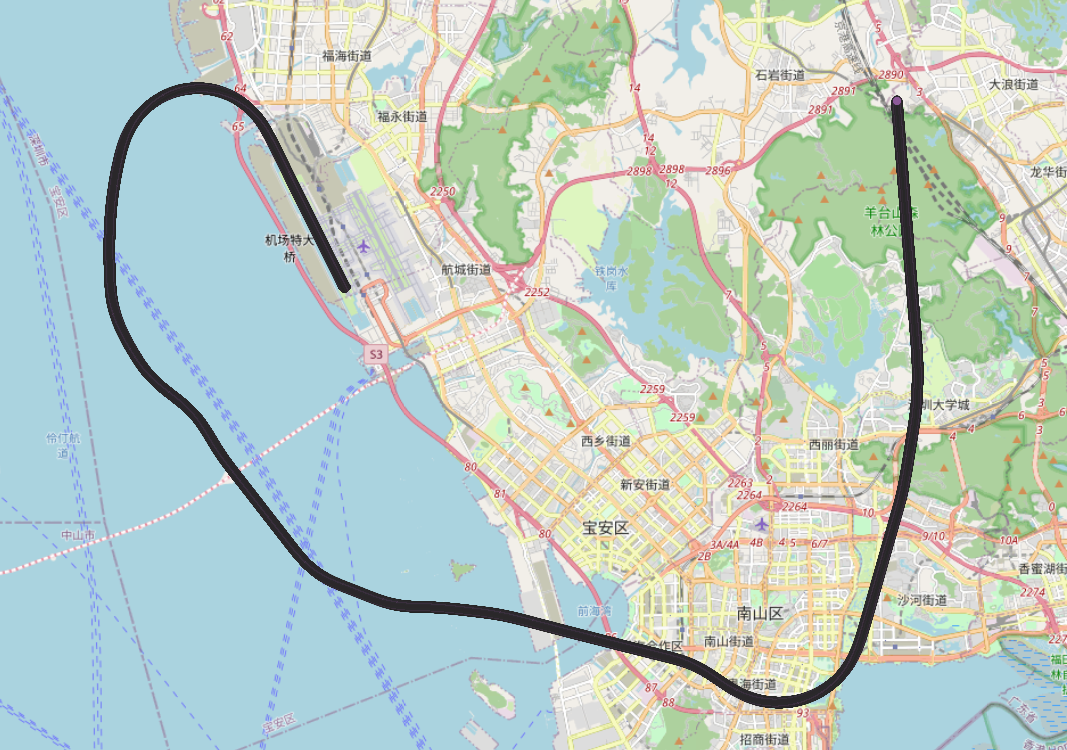
\includegraphics[width=.9\textwidth]{pictures/trace.png}
        \caption{GIS绘制路径}
        \label{GIStrace}
    \end{center}
\end{figure}
\begin{figure}[h!]
    \begin{center}
        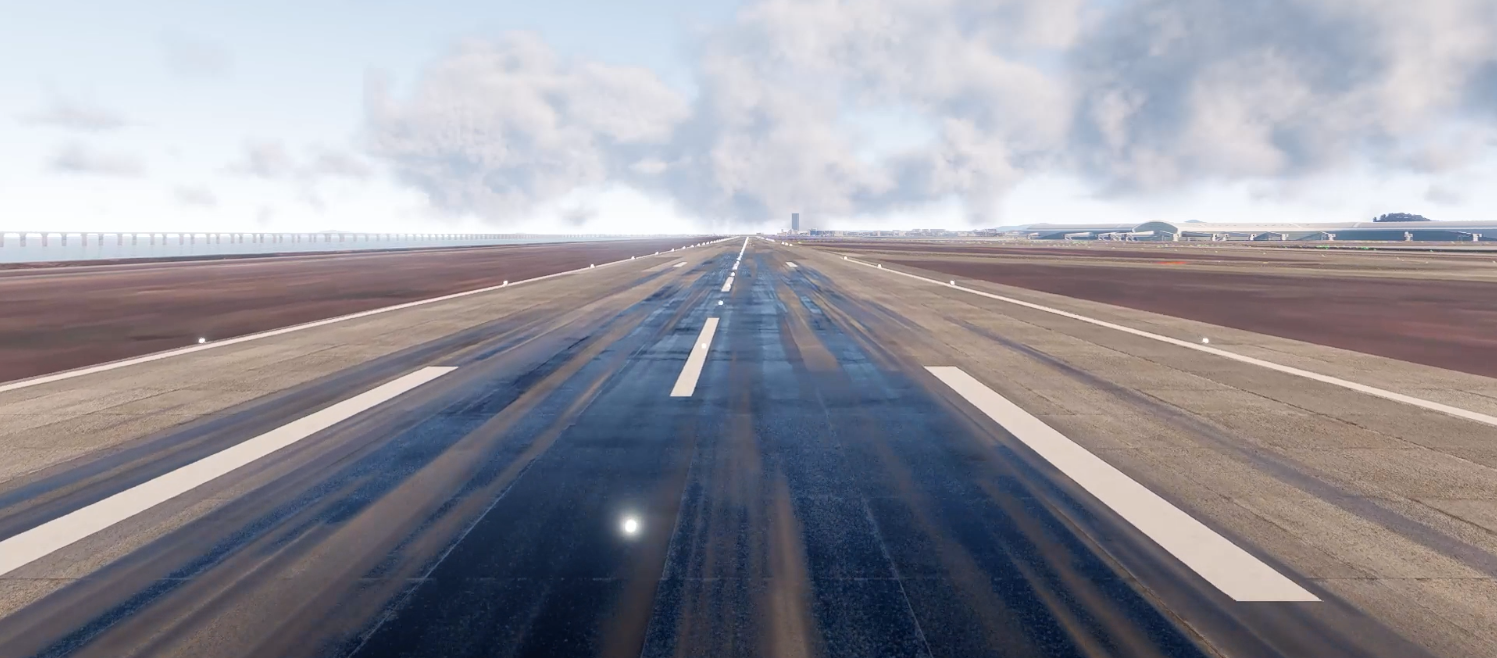
\includegraphics[width=.9\textwidth]{pictures/firstcamera.png}
        \caption{飞机第一视角}
        \label{firsttest}
    \end{center}
\end{figure}
\par
当摄像机位于第一视角下,按下X键即可切换为环绕视角。如图\ref{orbittest}所示,此时摄像机不在位于驾驶舱位置,而是在一定距离外始终看向驾驶舱。
鼠标左右方向的滑动可以改变Yaw角使摄像机水平方向的环绕,上下的滑动则改变Pitch角是竖直方向的环绕。经测试操作感受与主流游戏基本一致。
\clearpage
\begin{figure}[h!]
    \begin{center}
        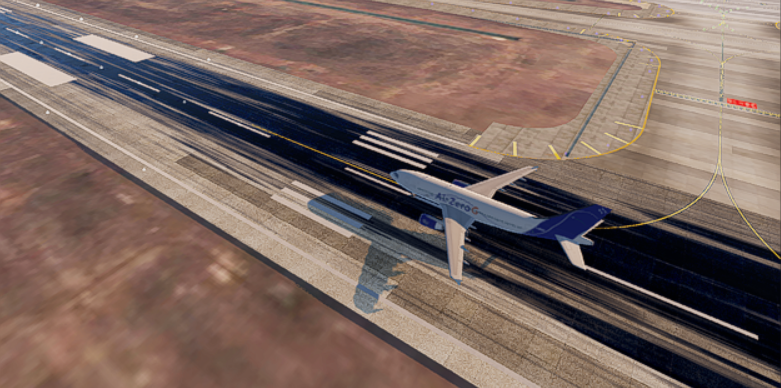
\includegraphics[width=0.9\textwidth]{pictures/orbitcamera.png}
        \caption{飞机环绕视角}
        \label{orbittest}
    \end{center}
\end{figure}
\par
当摄像机位于环绕视角下,按下X键即可切换为自由视角。如图\ref{freetest}所示,此时摄像机会在当前位置脱离飞机,并可以去到场景中的任意位置。
键盘的WASD键为前后左右移动,EQ键控制上下移动,这些移动方向都根据摄像机自身坐标系改变。Shift键则可以加速移动。经测试,操作感受与游戏引擎中的场景漫游基本一致。
\begin{figure}[h!]
    \begin{center}
        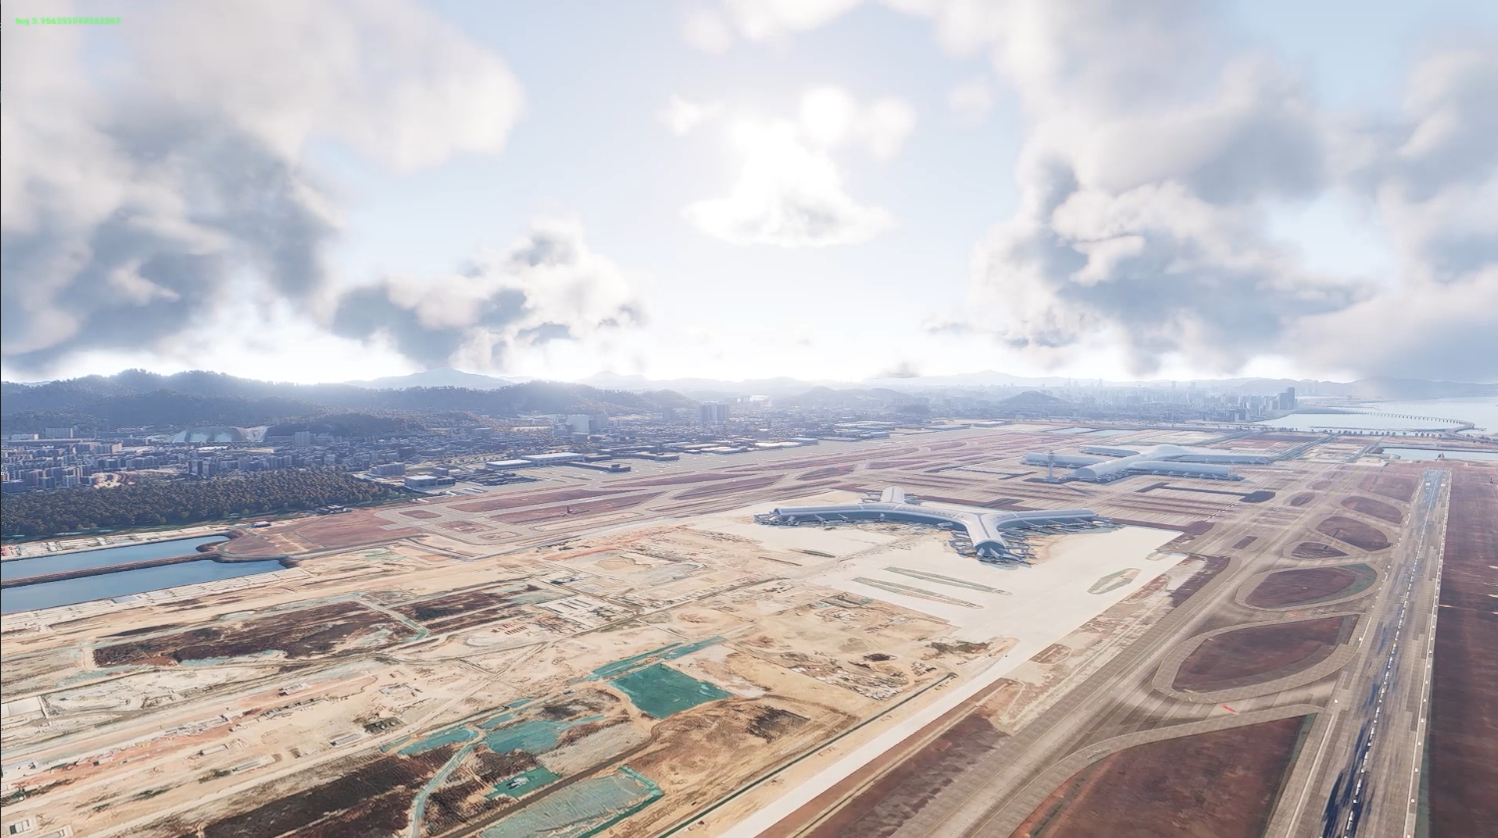
\includegraphics[width=.85\textwidth]{pictures/freecamera.png}
        \caption{自由视角}
        \label{freetest}
    \end{center}
\end{figure}
\par
飞机在飞行过程中会产生一些反馈信息,沿原路径最终送回仿真机。比如飞机在起飞和降落过程中会持续检测三个起落架的离地高度,
测试时便选用此信息,最终检查虚拟仿真机输出的原始数据包中此信息的值与训练基地FFS的反馈是否类似。
表\ref{fbcomp}对比了同一帧下CrossEngine和FFS关于起落架离地高度的反馈信息。由于地形资源存在些许差异,双方在此数据上并不会完全一致,
在合理范围内即可。
\begin{table}[h!]
    \begin{center}
        \caption{反馈信息对比}
        \label{fbcomp}
        \renewcommand\arraystretch{1.5}
        \begin{tabularx}{0.8\textwidth}{ 
             |>{\centering\arraybackslash\hsize=.7\hsize\linewidth=\hsize}X 
             |>{\centering\arraybackslash\hsize=1.15\hsize\linewidth=\hsize}X 
             |>{\centering\arraybackslash\hsize=1.15\hsize\linewidth=\hsize}X
             |
             }
             \hline 
            \textbf{起落架编号} & \textbf{CrossEngine} & \textbf{FFS}\\   
             \hline
             1 & 3.822m & 3.392m\\
             \hline
             2 & 3.787m & 3.368m\\     
             \hline
             3 & 3.787m & 3.368m\\
             \hline 
             ...& ... & ...\\
             \hline 
             1 & 40.031m & 39.894m\\
             \hline 
             2 & 39.914m & 39.785m\\
             \hline 
             3 & 39.912m & 39.785m\\
             \hline  
            \end{tabularx}
    \end{center}
\end{table}
\section{FFS环境测试}
真实FFS环境测试去到南方航空珠海基地,这里是亚洲最大,机型最全的模拟飞行训练基地,共拥有28台民航局运输司认证的最高D等级FFS,每年有超过7000名飞行员在此训练,是名副其实的中国民航飞行员培养摇篮。
在真实FFS环境中,主要对于与仿真机连接、飞机飞行等功能测试;同时对于帧率的稳定性进行测试。
\subsection{测试环境}
在真实FFS环境下虚拟仿真机与视景运行机同样位于两台电脑上,此时虚拟仿真机不再读取模拟数据,而是与仿真机进行交流,即可以接受飞行员的操作。
在硬件配置方面,基本为最新且性能最强的配件,保障视景流畅运行。在测试环境的具体物理配置信息如表\ref{ffshard}所示。
\clearpage
\begin{table}[h!]
    \begin{center}
        \caption{FFS环境物理配置}
        \label{ffshard}
        \renewcommand\arraystretch{1.5}
        \begin{tabularx}{\textwidth}{ 
             >{\centering\arraybackslash\hsize=.4\hsize\linewidth=\hsize}X 
             >{\centering\arraybackslash\hsize=.4\hsize\linewidth=\hsize}X 
             >{\centering\arraybackslash\hsize=\hsize\linewidth=\hsize}X 
             }
             \hline
            \textbf{设备} & \textbf{配置项} & \textbf{详情}\\         
             \hline
             & CPU & Intel® Core™ i9-12900K Processor\\
           
             & GPU & NVIDIA RTX A6000\\
             
             视景运行机 & 内存 & 64GB\\
            
             & 硬盘 & 8TB\\
             
             & 系统 & Windows 10 专业版 21H2\\
             \hline
             & CPU & Intel® Core™ i9-12900K Processor\\
           
             & GPU & Intel® UHD Graphics 770\\
             
             虚拟仿真机 & 内存 & 32GB\\
            
             & 硬盘 & 2TB\\
             
             & 系统 & Windows 10 专业版 21H2\\
             \hline
             
            \end{tabularx}
    \end{center}
\end{table}
\subsection{功能测试}
仿真机与虚拟仿真机通过网线连接。测试中启动与仿真机连接程序后,先选择要使用的网卡。连接建立成功后便可以开始正常接收数据。测试情况如图\ref{vsimcon}所示。
虚拟仿真机已成功读取到网卡上来自仿真机的原始数据包。
\begin{figure}[h!]
    \begin{center}
        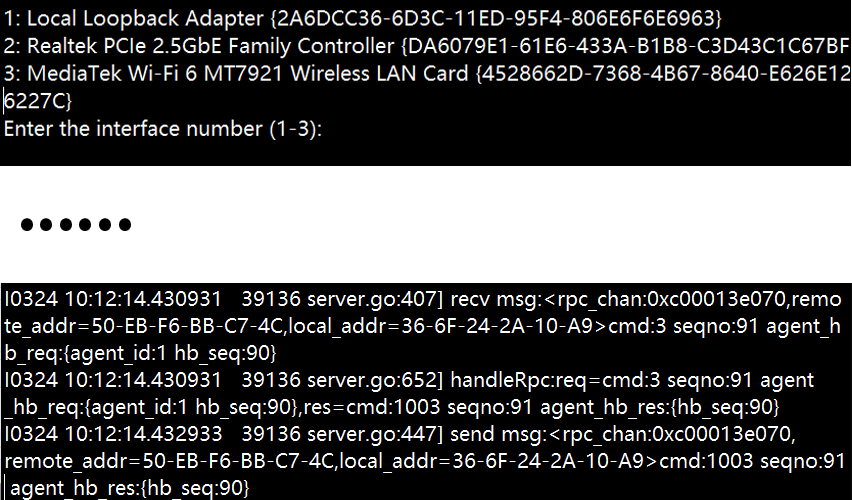
\includegraphics[width=.8\textwidth]{pictures/maclink.png}
        \caption{仿真机连接}
        \label{vsimcon}
    \end{center}
\end{figure}
\par
对于数据交换相关用例的测试同样是与服役中的FFS使用同一条预设路径飞行进行对比。本次测试选择的机场为广州白云机场,路径为跑道上的起飞过程。在服役FFS中运行的视频效果如图\ref{flightffs}所示,飞机即将在白云机场02L号跑道上完成起飞。
图\ref{flightffs}则展示了本视景系统运行该路径的情况,系统可以根据仿真机的数据正确将飞机初始位置置于机场02L号跑道,且在后续起飞过程中视景画面与上述服役FFS视频中完全一致。
目前画面仍存在球幕上的畸变问题以及颜色不准确的问题,但对于数据交换系统而言已经实现了核心功能。
\begin{figure}[h!]
    \begin{center}
        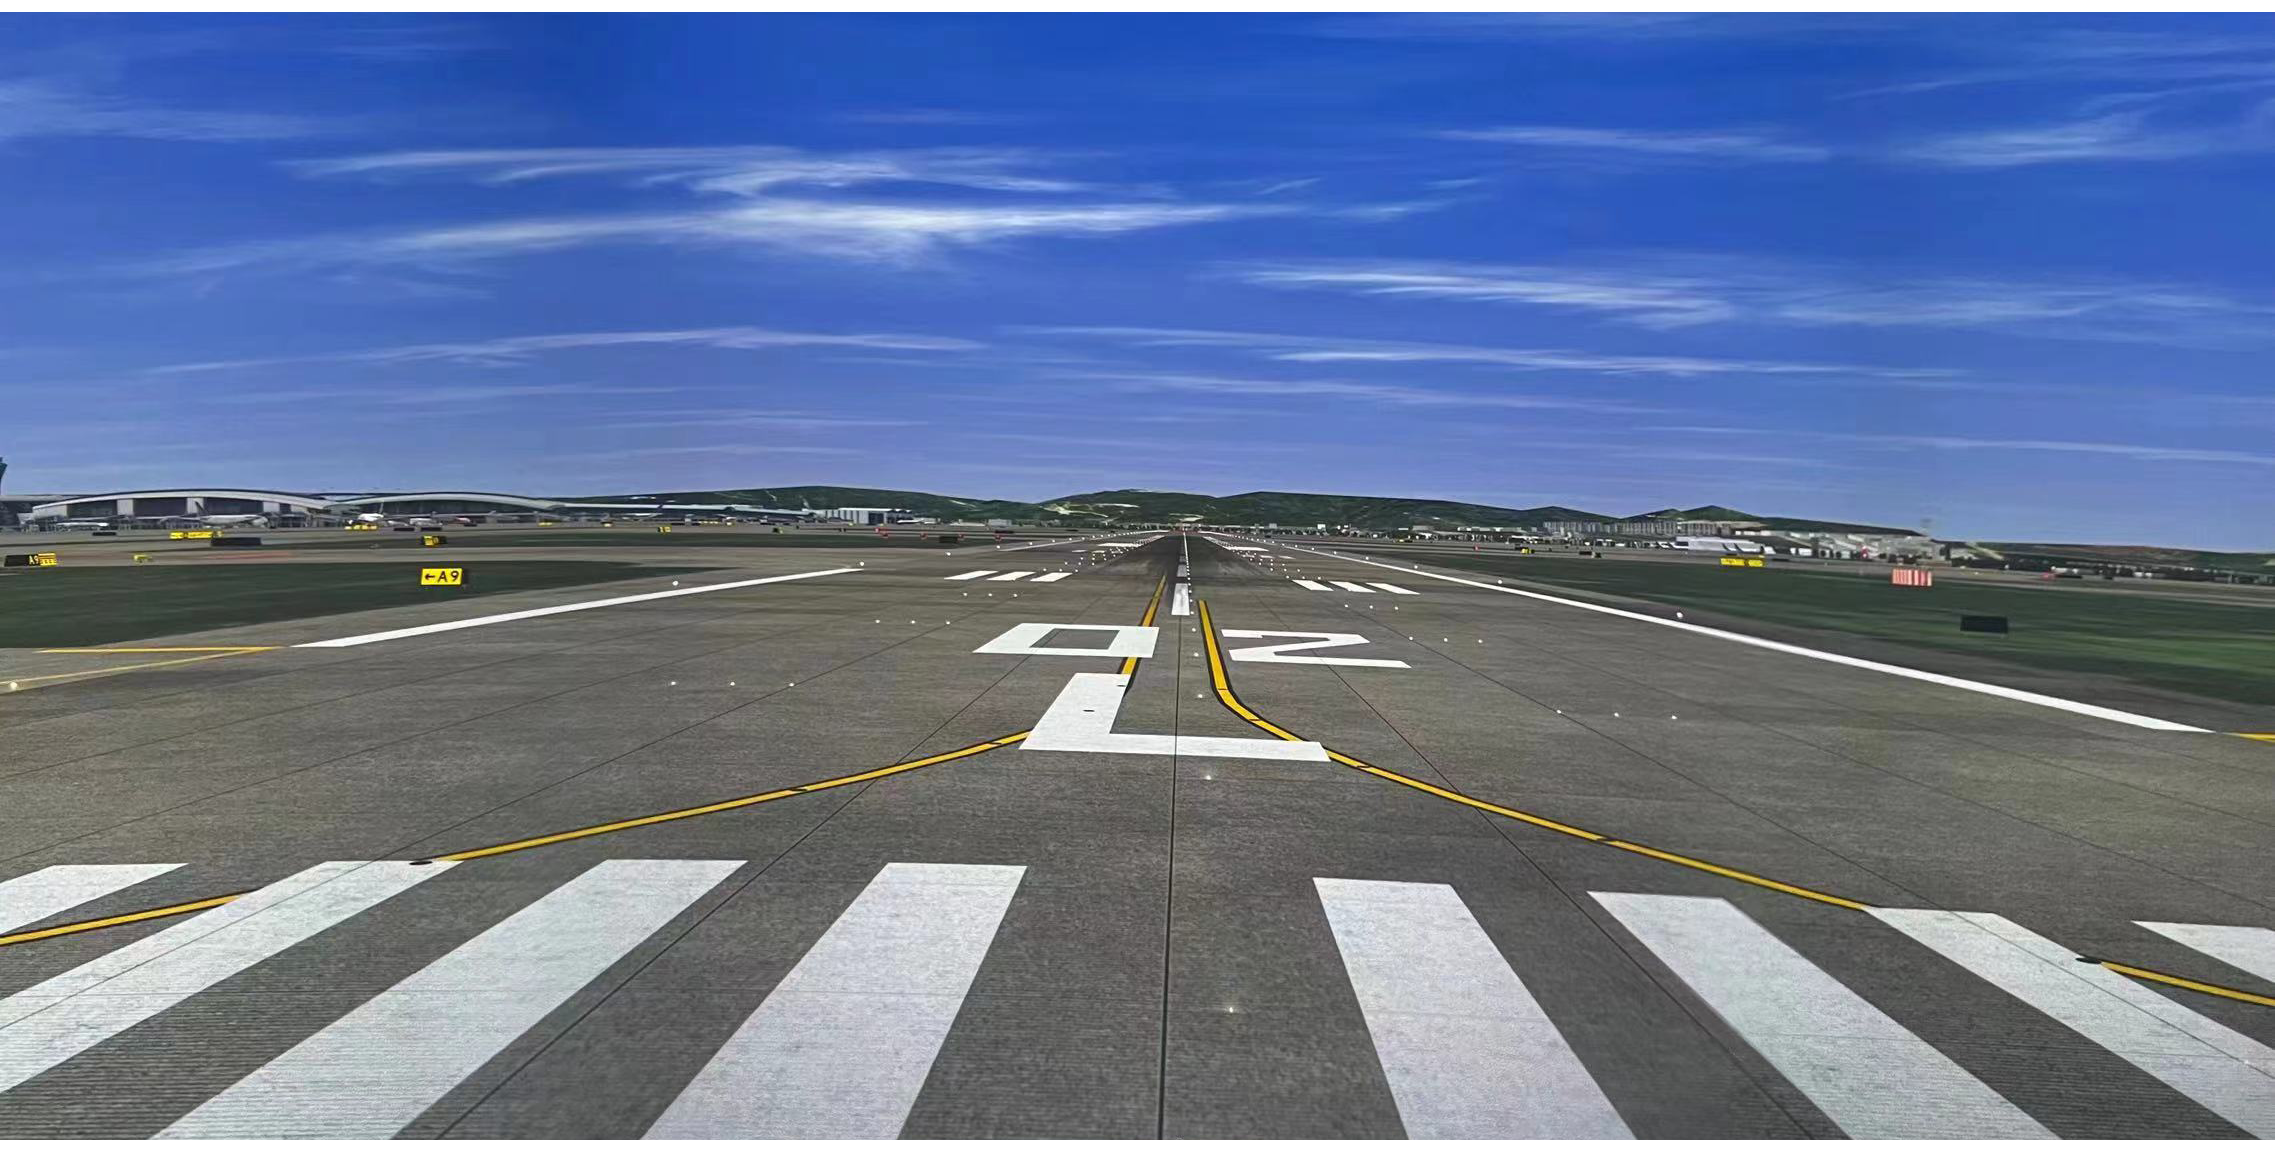
\includegraphics[width=.8\textwidth]{pictures/ffs2.png}
        \caption{服役中FFS运行效果}
        \label{flightffs}
    \end{center}
\end{figure}
\begin{figure}[h!]
    \begin{center}
        \includegraphics[width=.8\textwidth]{pictures/ffs.png}
        \caption{本视景系统运行舱内效果}
        \label{flighttest}
    \end{center}
\end{figure}
\subsection{性能测试}
性能测试的部分主要测试连续运行下视景系统的帧率稳定性。帧率检测使用第三方的监控软件,连续飞行一个小时,记录平均帧率、最高帧率、最低帧率和1\% Low帧的情况。
其中最高帧率与最低帧率并不是某一时刻的帧率,而是极短时间内的平均帧率。1\% Low是选取了帧生成时间最长的1\%的帧计算的平均帧率,这些帧不一定是连续的,所以一般会低于最低帧率,
表示整段测试时间内某些时刻的剧烈帧率波动。
\par
测试结果如表\ref{frametest}所示,视景系统限制帧率上限为60FPS,平均帧率十分接近这一数值,说明总体来讲基本能达到长时间运行下的帧率要求。
最高帧率60.8FPS说明对于帧率的限制较为成功。1\%Low距离平均帧率有较大的距离,说明在某些复杂场景下会产生比较剧烈的瞬时帧率波动。
\begin{table}[h!]
    \begin{center}
        \caption{帧率测试结果表}
        \label{frametest}
        \renewcommand\arraystretch{1.5}
        \begin{tabularx}{0.8\textwidth}{ 
             |>{\centering\arraybackslash\hsize=\hsize\linewidth=\hsize}X 
             |>{\centering\arraybackslash\hsize=\hsize\linewidth=\hsize}X 
             |
             }
             \hline 
            \textbf{项目} & \textbf{数值}\\   
             \hline
             运行时间 & 3612.015s\\
             \hline
             总帧数 & 212748 Frame\\     
             \hline
             平均帧率 & 58.9 FPS\\
             \hline 
             最低帧率& 48.6 FPS\\
             \hline 
             最高帧率& 60.8 FPS\\
             \hline 
             1\% Low& 28.1 FPS\\
             \hline  
            \end{tabularx}
    \end{center}
\end{table}
\section{本章小结}
本章首先介绍了系统测试,通过系统测试可以有效保证系统的质量,同时可以验证系统的可用性。
随后将测试分为了开发环境和真实FFS环境,分别作了部分功能测试,并由于硬件性能原因只在FFS环境中做了性能测试。
通过此测试可以证明系统满足需求分析中的功能需求,并在FFS环境中达成非功能需求。